\let\negmedspace\undefined
\let\negthickspace\undefined
\documentclass[journal]{IEEEtran}
\usepackage[a5paper, margin=10mm, onecolumn]{geometry}
%\usepackage{lmodern} % Ensure lmodern is loaded for pdflatex
\usepackage{tfrupee} % Include tfrupee package

\setlength{\headheight}{1cm} % Set the height of the header box
\setlength{\headsep}{0mm}     % Set the distance between the header box and the top of the text

\usepackage{gvv-book}
\usepackage{gvv}
\usepackage{cite}
\usepackage{amsmath,amssymb,amsfonts,amsthm}
\usepackage{algorithmic}
\usepackage{graphicx}
\usepackage{textcomp}
\usepackage{xcolor}
\usepackage{txfonts}
\usepackage{listings}
\usepackage{enumitem}
\usepackage{mathtools}
\usepackage{gensymb}
\usepackage{comment}
\usepackage[breaklinks=true]{hyperref}
\usepackage{tkz-euclide} 
\usepackage{listings}
% \usepackage{gvv}                                        
\def\inputGnumericTable{}                                 
\usepackage[latin1]{inputenc}                                
\usepackage{color}                                            
\usepackage{array}                                            
\usepackage{longtable}                                       
\usepackage{calc}                                             
\usepackage{multirow}                                         
\usepackage{hhline}                                           
\usepackage{ifthen}                                           
\usepackage{lscape}
\usepackage{tikz}
\usepackage{textcomp}
\usetikzlibrary{circuits.ee.IEC, positioning}
\begin{document}

\bibliographystyle{IEEEtran}
\vspace{3cm}

\title{6.6.23}
\author{Manognya Kundarapu - EE24BTECH11037
}
% \maketitle
% \newpage
% \bigskip
{\let\newpage\relax\maketitle}

\renewcommand{\thefigure}{\theenumi}
\renewcommand{\thetable}{\theenumi}
\setlength{\intextsep}{10pt} % Space between text and floats


\numberwithin{equation}{enumi}
\numberwithin{figure}{enumi}
\renewcommand{\thetable}{\theenumi}
\textbf{Question:} The normal to the curve $x^2=4y$ passing through $(1,2)$ is

\begin{enumerate}
    \item \textbf{Theoretical Solution:}\\ 
    Let the slope of the normal be 'm' at a point $(x_0,y_0)$ on the curve. We know;  
    \begin{align}
             \text{$2x_0=4$}\frac{dy}{dx}\\
        \implies m=\frac{-2}{x_0}\\
        \text{Equation of normal is given by }y-y_0=\frac{-2}{x_0}(x-x_0)\\
       \text{Substituting (1,2) in above }2-y_0=\frac{-2}{x_0}(1-x_0)\\
       \text{also } (x_0)^2=4y\\
        \text{On solving we get }x_0=2,y_0=1\\
        \implies \text{required normal is } x+y=3
    \end{align}
    \item \textbf{Using Gradient descent method: }\\ 
    We want to find the normal line to the curve $x^2=4y$ at a specific point $(x_0,y_0)$, such that this normal passes through the point (1,2).\\
    
    Thus, if we know the coordinates $(x_0,y_0)$,  we can form the equation of the normal using point-slope form: $(y-y_0)=\frac{-2}{x_0}(x-x_0)$\\ $\implies y=mx+b$\\
    
    \textbf{Objective function (Minimization goal): }\\
    We want to minimize the distance between the point (1,2) and the normal line. In other words, we want to find the point $(x_0,y_0)$ on the curve where the normal passes through the point (1,2).\\
    
    $\implies d = \frac{|y_0-mx_0-b|}{\sqrt{1+m^2}}$\\

    \textbf{Gradient descent: }\\Gradient descent is an optimization algorithm used to minimize a function iteratively. Here's how it works:\begin{itemize}
        \item We start with an initial guess for $(x_0,y_0)$
        \item We compute the gradient (partial derivatives) of the objective function with respect to $x_0$ and $y_0$
        \item We update $x_0$ and $y_0$ in the direction that reduces the distance (minimizes the objective function).
        \item This is done iteratively until the values converge to a point where the gradient is close to zero (indicating a minimum).
    \end{itemize}
\textbf{Steps in the Gradient Descent Algorithm:}
    \begin{itemize}
        \item Start with initial guesses for $x_0$ and $y_0$ (we chose $x_0=2, y_0=1$ as a starting point).
        \item The gradient of the objective function tells us how to change $x_0$ and $y_0$ to minimize the distance. In the gradient descent process, we calculate the partial derivatives of the distance with respect to $x_0$ and $y_0$
        \item  Adjust $x_0$ and $y_0$ by a small amount in the direction of the negative gradient (i.e., move in the direction that reduces the distance).
        \[
x_0 \leftarrow x_0 - \text{learning rate} \times \frac{\partial \text{Distance}}{\partial x_0}
\]

\[
y_0 \leftarrow y_0 - \text{learning rate} \times \frac{\partial \text{Distance}}{\partial y_0}
\]
\item Continue this process for a set number of iterations or until the changes become very small (i.e., convergence)
\end{itemize} The below graph shows the comparison between the curve that is obtained theoretically and the simulation curve(numerically generated points through iterations).
\end{enumerate}
\begin{figure}[htbp]
  \centering
  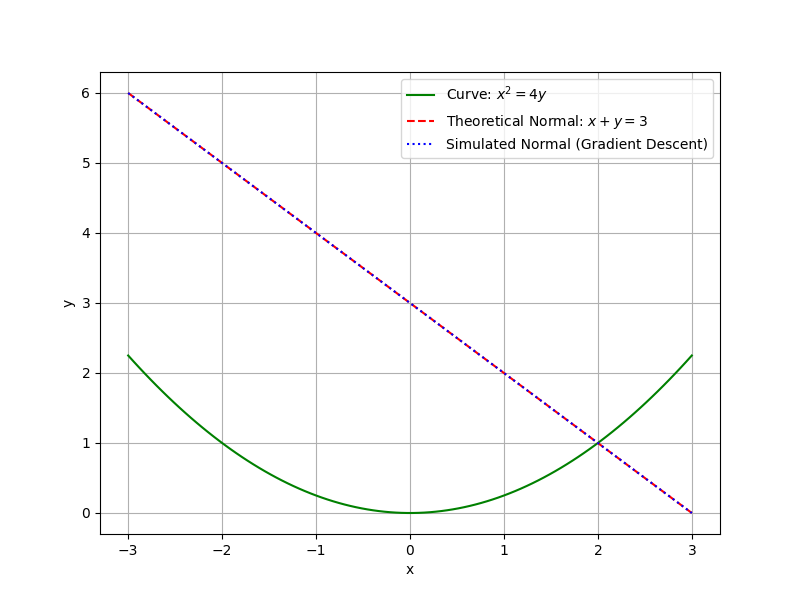
\includegraphics[width=\columnwidth]{figs/curve.png}
\end{figure}

\end{document}
